% Definiciones y constantes de estilo
% Clase del documento
\documentclass[a4paper,12pt,twoside,openright,titlepage]{book}

%
% Paquetes necesarios
%

% Codificación UTF8
\usepackage[utf8]{inputenc}
% Title
\usepackage{titling}
% Márgenes
\usepackage[hmargin=3cm,vmargin=3.5cm]{geometry}
% Definición de colores
\usepackage{color}
% Extensión del paquete color
\usepackage[table,xcdraw,dvipsnames]{xcolor}
% Cabecera y pie de página
\usepackage{fancyhdr}
% Estilo título capítulos
\usepackage{quotchap}
% Títulos de secciones
\usepackage{titlesec}
% Enumeraciones
\usepackage{enumerate}
% Páginas en blanco
\usepackage{emptypage}
% Código, algoritmos, etc.
\usepackage{listings}
% Separación entre cajas
\usepackage{float}
% Imágenes
\usepackage[pdftex]{graphicx}
% Incluir pdfs externos
\usepackage{pdfpages}
% Apéndices
\usepackage{appendix}
% Marcadores (para el pdf)
\usepackage{bookmark}
% Estilo de enumeraciones
\usepackage{enumitem}
% Espacio entre líneas y párrafos
\usepackage{setspace}
% Glosario/Acrónimos
\usepackage[acronym]{glossaries}
% Fuentes
\usepackage[T1]{fontenc}

% Subtitle
\newcommand{\subtitle}[1]{%
	\posttitle{%
		\par\end{center}
		\begin{center}\large#1\end{center}
		\vskip0.5em
		}%
}

% Enlaces
\hypersetup{hidelinks,pageanchor=true,colorlinks,citecolor=Fuchsia,urlcolor=black,linkcolor=Cerulean}

% Euro (€)
\DeclareUnicodeCharacter{20AC}{\euro}

% Inclusión de gráficos
\graphicspath{{./images/}}

% Extensiones de gráficos
\DeclareGraphicsExtensions{.pdf,.jpeg,.jpg,.png}

% Definiciones de colores (para hidelinks)
\definecolor{LightCyan}{rgb}{0,0,0}
\definecolor{Cerulean}{rgb}{0,0,0}
\definecolor{Fuchsia}{rgb}{0,0,0}

% Estilo páginas de capítulos
\fancypagestyle{plain}{
\fancyhf{}
\fancyfoot[CO]{\thepage}
\renewcommand{\footrulewidth}{.6pt}
\renewcommand{\headrulewidth}{0.0pt}
}

% Estilo resto de páginas
\pagestyle{fancy}

\renewcommand\thesection{\arabic{section}}

% Guía del pie de página
\renewcommand{\footrulewidth}{.6pt}

% Nombre del titulo para indice de codigo
\renewcommand\lstlistlistingname{Table of code}

% Nombre de los bloques de código
\renewcommand{\lstlistingname}{Code}

% Estilo de los lstlistings
\lstset{
    frame=tb,
    breaklines=true,
    showstringspaces=false,
    postbreak=\raisebox{0ex}[0ex][0ex]{\ensuremath{\color{gray}\hookrightarrow\space}}
}

% Definiciones de funciones para los títulos
\newlength\salto
\setlength{\salto}{3.5ex plus 1ex minus .2ex}
\newlength\resalto
\setlength{\resalto}{2.3ex plus.2ex}

% Estilo de los acrónimos
\renewcommand{\acronymname}{Acronym}
\renewcommand{\glossaryname}{Acronym}
\pretolerance=2000
\tolerance=3000

% Comando code (lstlisting sin cambio de página)
\lstnewenvironment{code}[1][]%
  { \noindent\minipage{0.935\linewidth}\medskip
    \vspace{5mm}
    \lstset{basicstyle=\ttfamily\footnotesize,#1}}
  {\endminipage}

% Numerado hasta sub subsecciones
\setcounter{secnumdepth}{3}

\title{Commercial flights delay prediction}
\subtitle{Máster Universitario en Ingeniería Informática\\
		  Universidad Politécnica de Madrid}
\author{José Domínguez Pérez\\
		Ismael Muñoz Aztout\\
		Jonatan Ruedas Mora}
\date{December 2020}

\makeindex
\begin{document}
\maketitle
\tableofcontents
\newpage

\section{Introduction}

For this analysis we have developed two projects.

\begin{itemize}

	\item The first one has been developed in the R programming language. In this project we perform an exploratory data analysis to investigate which variables are related to our target variable. This project contains the source code in which we carry out the processing and visualization of the dataset and a folder called plots where the plots of the analysis are saved.

	\item The second one is the Spark project that is requested in this practical work. It is written in Scala and is the project where we load and process the data to create a machine learning model that can predict the delays of commercial flights. The project follows the structure of a Maven project.
	
\end{itemize}

\section{Analysis}

Once we have explained how our practical work is structured, we will explain how we carry out the exploratory analysis of the data to select the useful variables.\\

To do this, we cleaned several values of the dataset like the forbidden variables and the variables that we have considered useless (\textit{Cancelled} and \textit{CancellationCode}). We also have created a new column called \textit{Date} that merges the \textit{Year}, \textit{Month} and \textit{DayofMonth} variables. Later, we have factorized the categorical values in order to prepare them to generate the correlation matrix. Apart from that, instead of omitting the NA values we gave a value of 0 to all the missing values because in some datasets (i.e., 1987) there were some related columns that were full of them.\\

When we were sure that the data was correctly cleaned we proceeded to generate the correlation matrix in which we could see which variables were strongly correlated with our target variable. As a result, we decided to use only the 2 most correlated variables because the other correlation values were quite low.\\

\begin{figure}[H]
	\centering
	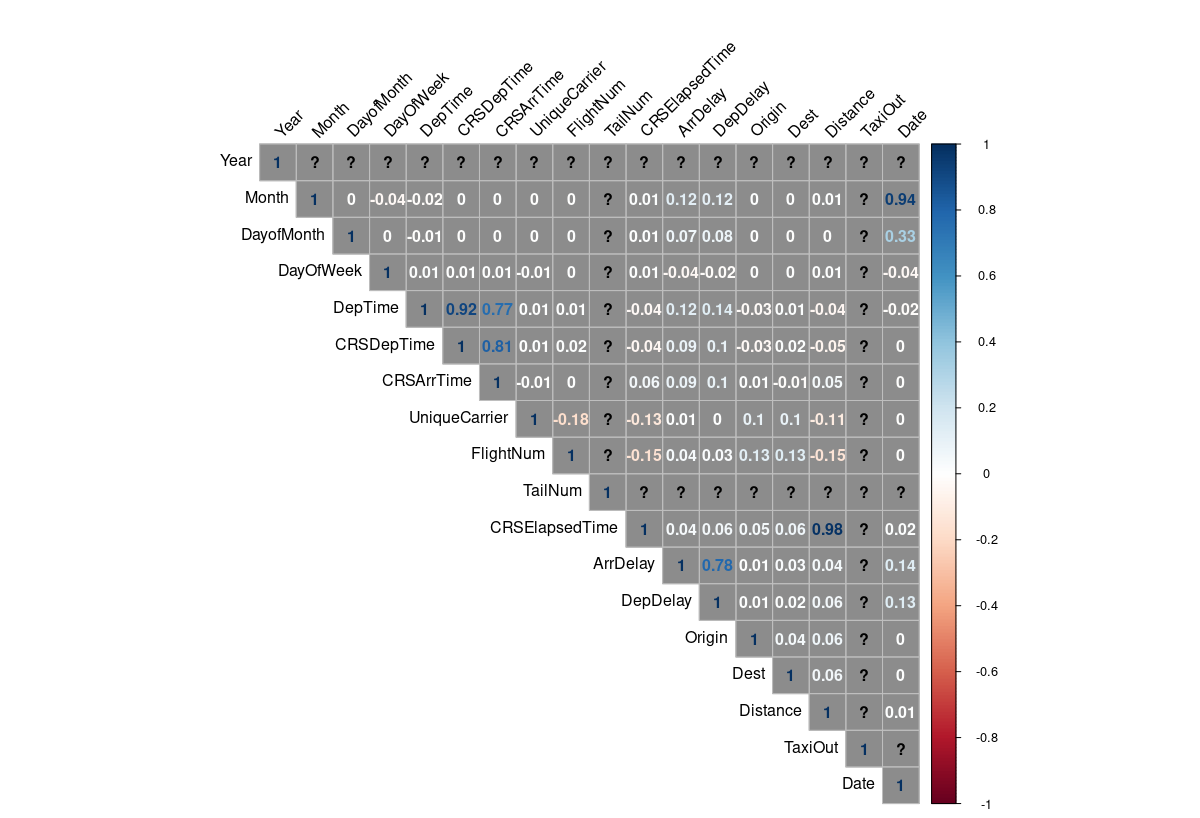
\includegraphics[scale=.4]{1987_corr_matrix}
	\caption{1987 correlation matrix}
\end{figure}

\begin{figure}[H]
	\centering
	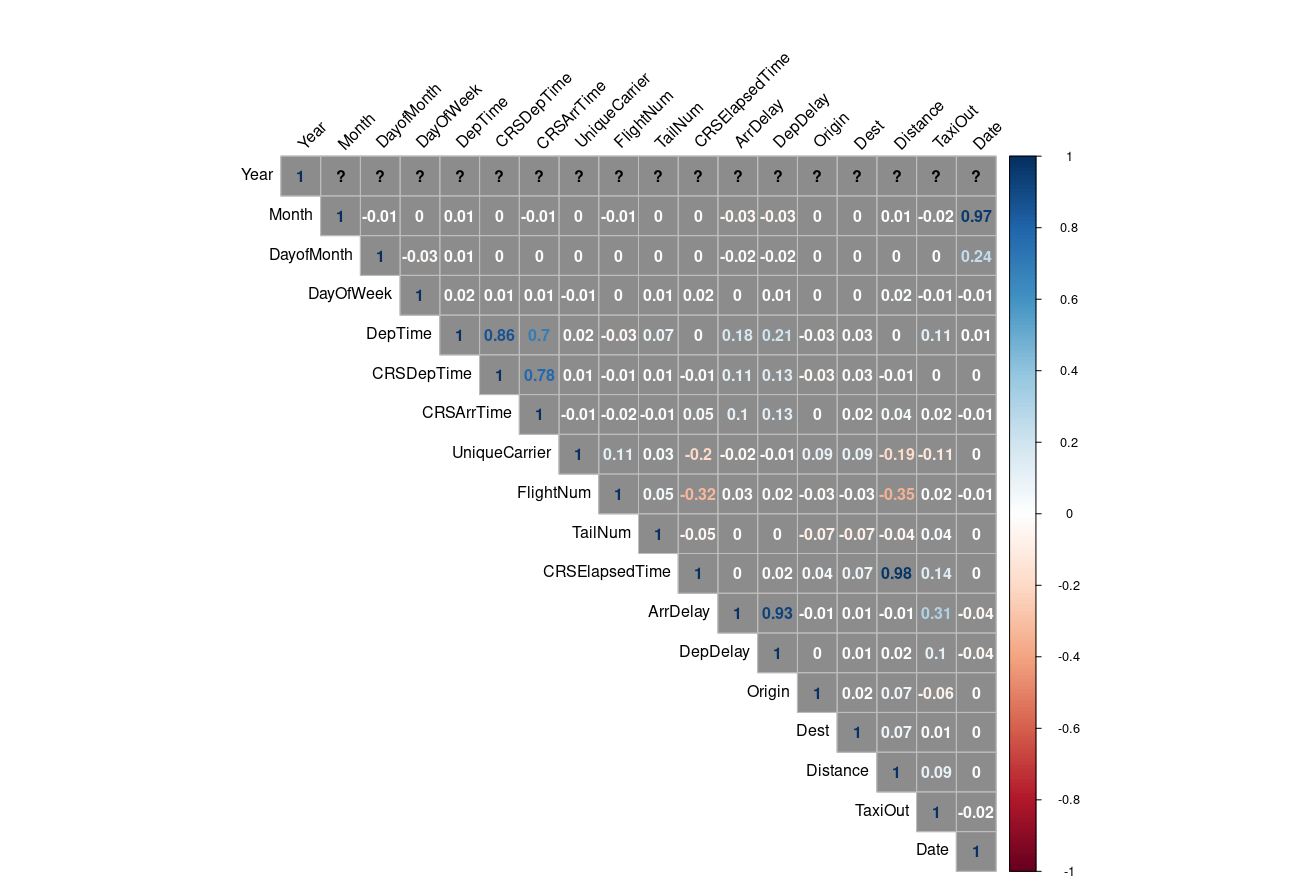
\includegraphics[scale=.4]{2008_corr_matrix}
	\caption{2008 correlation matrix}
\end{figure}

After that, we generated a scatterplot for the 2 selected variables to see how they correlate with the target variable. We realized that in some datasets, like 1987, the TaxiOut variable was full of NA values but when it does have value it influences the ArrDelay so we decided to keep that variable and use it to build the model. The figure \ref{fig:1987_taxi_out} shows that graphic because we used 0 to replace NA and the column only had missing values. \\

\begin{figure}[H]
	\centering
	\begin{minipage}{.45\textwidth}
		\centering
		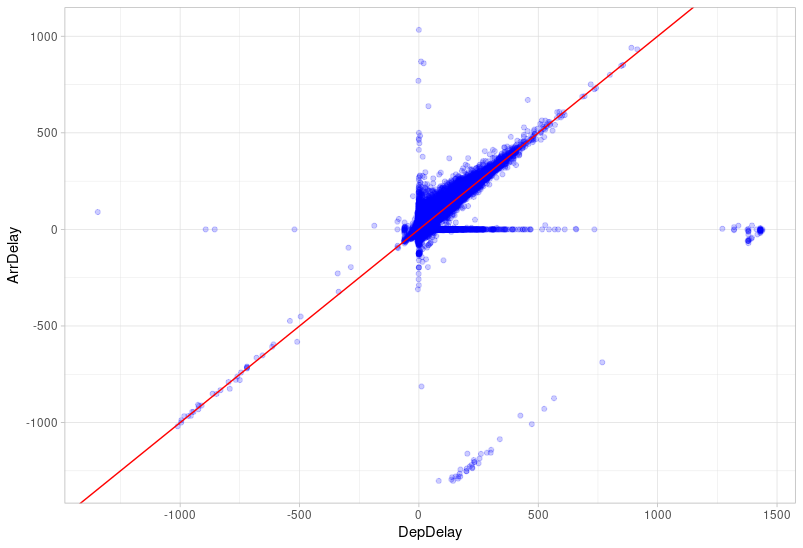
\includegraphics[width=1\textwidth]{1987_dep_delay}
		\caption{1987 ArrDelay vs DepDelay}
		\label{fig:1987_dep_delay}
	\end{minipage}\hfill
	\begin{minipage}{.45\textwidth}
		\centering
		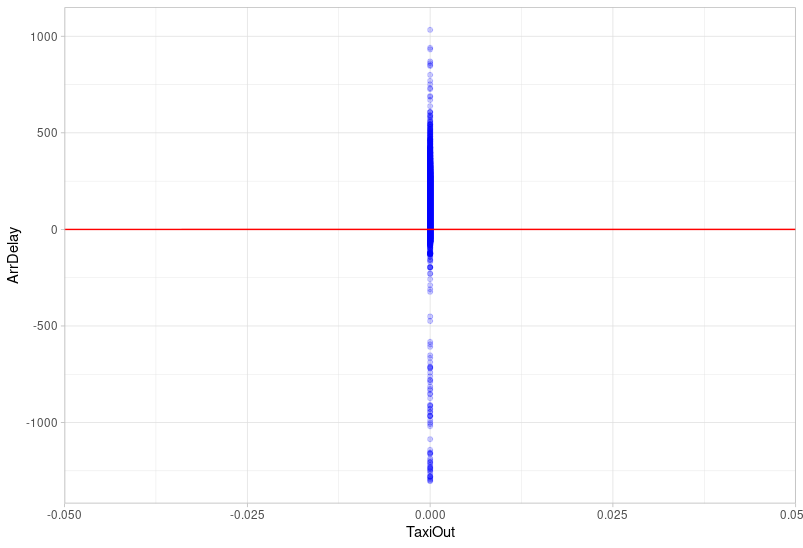
\includegraphics[width=1\textwidth]{1987_taxi_out}
		\caption{1987 ArrDelay vs TaxiOut}
		\label{fig:1987_taxi_out}
	\end{minipage}
\end{figure}

\begin{figure}[H]
	\centering
	\begin{minipage}{.45\textwidth}
		\centering
		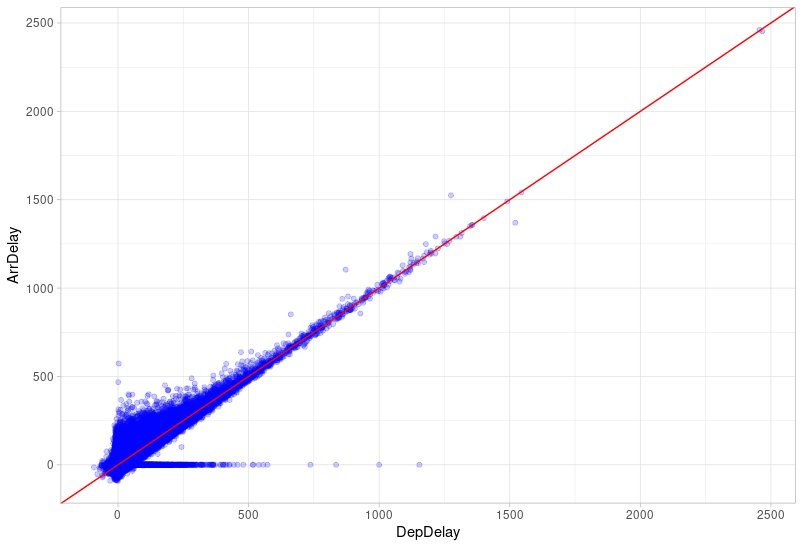
\includegraphics[width=1\textwidth]{2008_dep_delay}
		\caption{2008 ArrDelay vs DepDelay}
		\label{fig:2008_dep_delay}
	\end{minipage}\hfill
	\begin{minipage}{.45\textwidth}
		\centering
		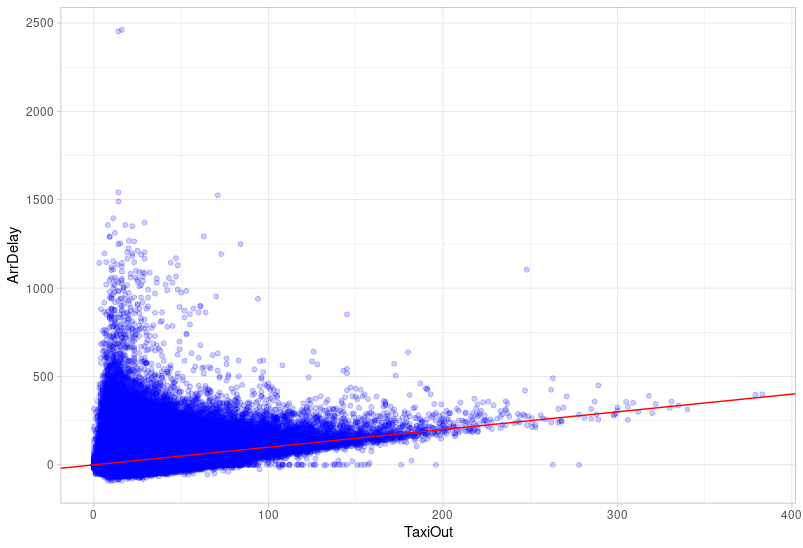
\includegraphics[width=1\textwidth]{2008_taxi_out}
		\caption{2008 ArrDelay vs TaxiOut}
		\label{fig:2008_taxi_out}
	\end{minipage}
\end{figure}

\subsection{Insights}
After carrying out different tests with different datasets, we decided to use the DepDelay and TaxiOut variables in order to make our prediction for the aforementioned reasons, discarding the rest of the variables as they have a very low correlation index or they were not correlated at all.

\section{Variable selection}

\subsection{Selected variables}
We have selected the following variables:

\begin{itemize}
	\item \textit{DepDelay}
	\item \textit{TaxiOut}
\end{itemize}

\subsection{Excluded variables}
Forbidden variables:

\begin{itemize}
	\item \textit{Arrtime}
	\item \textit{ActualElapsedtime}
	\item \textit{AirTime}
	\item \textit{TaxiIn}
	\item \textit{Diverted}
	\item \textit{CarrierDelay}
	\item \textit{WeatherDelay}
	\item \textit{NASDelay}
	\item \textit{SecurityDelay}
	\item \textit{LateAircraftDelay}
\end{itemize}

Categorical variables have been factorized in order to have numerical variables. These variables are:

\begin{itemize}
	\item \textit{UniqueCarrier}
	\item \textit{TailNum}
	\item \textit{Origin}
	\item \textit{Dest}
\end{itemize}

The \textit{Cancelled} and \textit{CancellationCode} variables has been excluded because when a flight is cancelled, it will not arrive to the destination and it will be useless to predict arrival delay.\\

When cleaning the dataset in Scala, we remove all of the forbidden variables and what we call \textit{useless} variables that are the ones that have a weak level of correlation (under 0.25 more or less) with the target variable.

\subsection{Transformed variables}
We have transformed the categorical variables in our dataset into numbers by factorizing them. This way, we can assign them a numerical value in order to perform calculations such as correlation.

\subsection{Created variables}
We have created a new column called \textit{Date} that merges the \textit{Year}, \textit{Month} and \textit{DayofMonth} variables but we discarded later because it was not correlated to the target variable.

\section{Machine learning model}

\subsection{Selected techniques}

First of all, our target variable is continuous and we have its actual value (supervised learning), so we have selected some regression algorithms. These algorithms are as follows:

\begin{itemize}

	\item \textbf{Linear Regression}, which is a basic and commonly used type of predictive analysis and the main reasons why we have chosen this algorithm are:

	\begin{itemize}
		\item Provides good predictive results of the target variable with respect to the set of predictor variables.
		
		\item It is one of the best known algorithms and we are familiar with it after having used it in various subjects.
	\end{itemize}		
	
	\item \textbf{Gradient Boosted Tree}, which is one of the most powerful techniques for building predictive models. BTs iteratively train decision trees in order to minimize a loss function. Like decision trees, GBTs handle categorical features, extend to the multiclass classification setting, do not require feature scaling, and are able to capture non-linearities and feature interactions. The main reason why we have chosen this algorithm is:
	
		\begin{itemize}
			\item To be able to compare the results of both algorithms, where it can be verified that the linear regression algorithm is much better than GBT.
		\end{itemize}	
	
\end{itemize}

\subsection{Validation process}

The process of validation we have used in order to measure the accuracy of the selected machine learning algorithm is as follows:\\

Firstly, we have divided our dataset into two parts:

		\begin{itemize}
			\item The \textbf{training set}: used to train our data. 
			\item The \textbf{test set}: used to assess the actual performance of the chosen algorithm. When training the dataset, we are provided with different metrics that can be used to validate our model. However, these metrics are calculated based on the training data and we need to ensure that this algorithm is also accurate with respect to independent data that has not been used in the training step. This is why we keep a part of the dataset that has not been used for training.
		\end{itemize}
		
Secondly, apart from splitting out the dataset into the training and test dataset, we also divide the training part into different validation sets in order to conduct cross-validation. This validation process is used to find the best parameters for our machine learning algorithm, which is also called hyper-parameter tuning. This way, we can select the best parameters for our model before assessing its performance with the test data. More specifically, we are going to make use of the K-fold cross-validation, where training data is randomly partitioned into K equal sized subsets that are used to validate the remaining training data. Next, we will show an illustration to clarify the whole process of validation we have implemented. In this example, a K-fold cross-validation of K=5 has been used.\\

\begin{figure}[H]
	\centering
	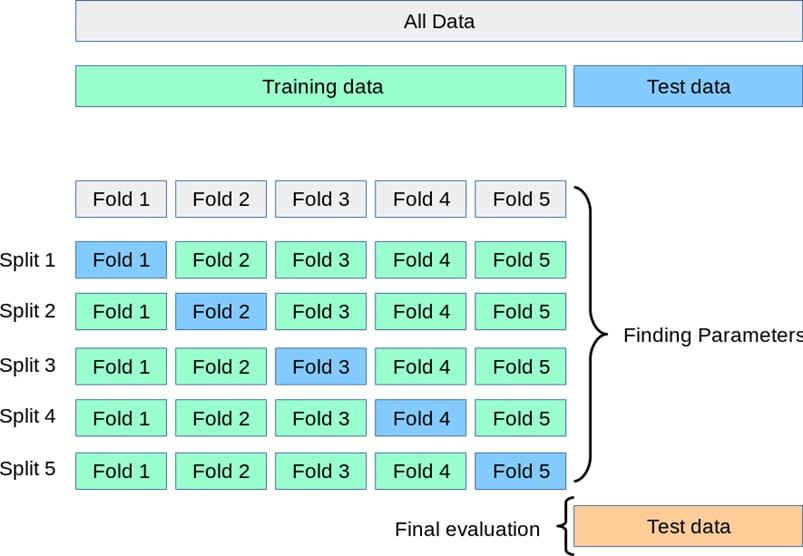
\includegraphics[scale=.8]{validation}
	\caption{Validation process}
\end{figure}

Once we have found the parameters that best fit the model, we can use these parameters to assess the actual accuracy of our model by evaluating it with the test set. Next, we will discuss the metrics we have used to assess the accuracy of the models. As we have implemented regression algorithms in order to predict the target variable (since this variable is continuous), we have used the following regression metrics:

\begin{itemize}

	\item Mean Squared Error (\textbf{MSE}): this metric measures the average squared difference between the estimated and actual values.
	
	\item Root Mean Squared Error (\textbf{RMSE}): this metric measures the average difference between the estimated and actual values.
	
	\item Mean Absolute Error (\textbf{MAE} ): this metric measures the average difference between the estimated and actual values, without considering their directions.
	
	\item Coefficient of determination (\textbf{R\textsuperscript{2}}): this metric measures “how well” our predictor variables explain the target variable. The values of this metric ranges from 0 (when predictor variables cannot explain the target variable) to 1 (when predictor variables explain the target variable at its best).

\end{itemize}

Finally, we are going to discuss what regression metrics we have chosen and why.\\

Firstly, the coefficient of determination is a very useful metric when assessing the accuracy of a model due to the fact that the value of this coefficient always ranges from 0 to 1, regardless the type of algorithm. However, it does not provide us with an idea of the \textbf{magnitude} of the error. This is why we have discarded this metric.\\

Then, we have the first 3 metric errors, which are very similar metrics that tell us the magnitude of the error. The difference between these metrics is that the MSE provide us with the average squared error instead of the average error, so we can also discard it. Now we have to choose between the RMSE and the MAE. The main difference between these last two metrics is that the RMSE gives a higher weight to large errors, which are commonly undesirable. So this is why we have chosen the \textbf{RMSE} metric.

\subsection{Model evaluation}

The results that we have obtained using the dataset of the year 2008 are these.

\begin{figure}[H]
	\centering
	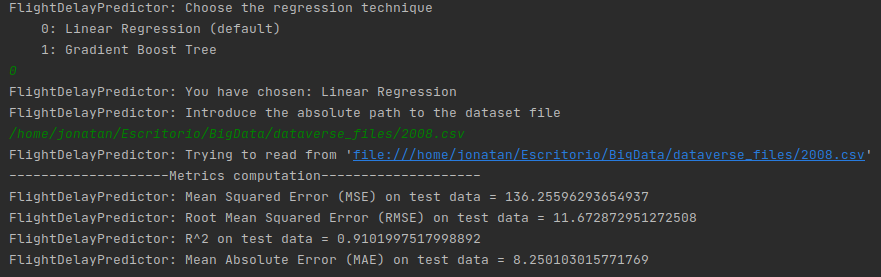
\includegraphics[scale=.8]{result_2008_linear}
	\caption{Linear Regression result}
\end{figure}

\begin{figure}[H]
	\centering
	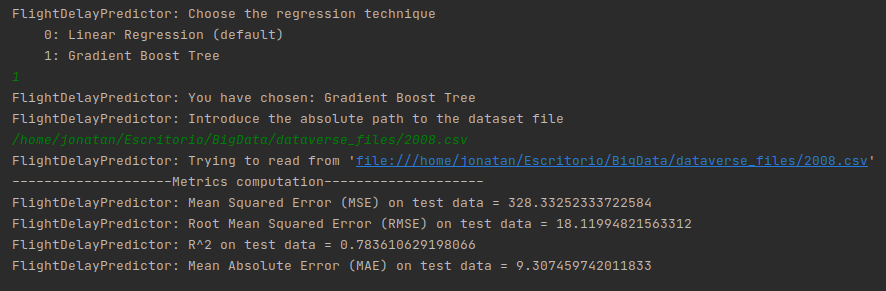
\includegraphics[scale=.8]{result_2008_gbt}
	\caption{Gradient Boosted Tree result}
\end{figure}

As we can see, the linear regression algorithm is much more precise than the GBT algorithm due to the fact that the RMSE for the linear regression is almost half of the GBT. Also, we can see that all of the others metrics are better for the linear regression model.\\

Therefore, we can conclude that it would be much more optimal to use the linear regression to deduce our target

\section{Execution instructions}

To be able to run out app, you only have to press the run button. After that choose which algorithm you want to test and put the path where the data collection is in cvs format.

\subsection{Input data}

You do not need to have a specific location where the data set is, the only thing you should keep in mind is to put the correct path to run the app.

\subsection{ML technique selection}

We have 2 possible techniques to perform the model construction, Linear Regression and Gradient Boosted Tree. You have to select one of those techniques using the keyboard numbers 0 or 1. By default Linear Regression will be used.

\begin{figure}[H]
	\centering
	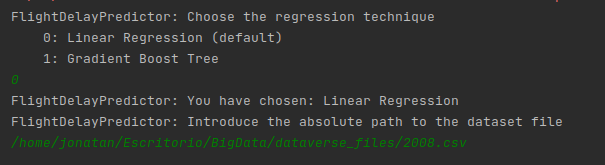
\includegraphics[scale=.8]{app_start}
	\caption{App start parameters}
\end{figure}

\subsection{Error handling}

We check some errors like empty folders, not \textit{.csv} file or wrong technique selection, those errors are managed through exceptions and terminate the execution of the program.

\section{Final conclusions}

We found this project very interesting, in addition to be able to get a little fluency programming spark looking information in the notes of this subject and the official pages of spark. The main problem was the statistical aspect because we do not have advanced background about this field, even though, this project has been educative and interesting.

\end{document}